\chapter{Alternatives to Dark Energy}

%\begin{doublespace}

\section{Introduction}

It is important for researchers in dark energy, and cosmology in general, to be familiar with the observational basis for claims regarding the most appropriate cosmological model. Perhaps the weakest link in the chain of observation and reasoning leading to the LCDM model, lies in the assumptions used to determine luminosity distances between Earth and the various astronomical objects that serve as ``standard candles". These calculations are commonly done with the assumption of large-scale homogeneity in the visible universe. Recent evidence (\cite{York2000The-Sloan,Abazajian2009The-Seventh,Percival2001The-2dF-Galaxy}) highlighting the complexity in the large-scale structure (\cite{vandeWeygaert2009Geometry,vandeWeygaert2004Hierarchy,Shandarin2004Morphology}), conclusively demonstrates that we live in a universe whose evolution during the current epoch cannot be described by linear perturbation theory. Such an approach is applicable from the time of the last scattering surface ($ t_{rec}$) upto the earliest stages of star and galaxy formation ($ t_{struct} $). Past that stage, regions with a large enough density contrast have formed whose further evolution requires non-linear methods along the lines of those used to describe dark matter halo evolution (\cite{Giocoli2007An-improved}) . Once regions with large enough density contrast\footnote{$ |1-\rho/\overline{\rho}| \gtrsim 0.1 $; the ratio between the local matter density and the large-scale averaged density} have formed the next phase in the evolution involves processes of collisions between these regions, leading to the formation of galaxy clusters connected by filaments of matter, a structure collectively referred to today as the ``Cosmic Web".

This magnificent structure can be thought as the scaffolding of our universe. It resembles a foam-like fluid containing voids (regions of under-density) between which are sandwiched sheets of matter forming one-dimensional filamentary structures which join up at cosmic ``nodes" which can be identified as regions with active star formation.

One reason for the success of the LCDM model is that the propagation of light through these complex structures appears to be an analytically intractable problem. Various arguments have been made in the literature [\textbf{find and cite refs}] justifying the assumption of homogeneity, even though regions with a density contrast as high as $ \pm 0.3 $ are known to exist in our cosmic neighborhood. For the greater portion of the time it takes a photon to travel from $ t_{rec} $ to the present epoch, it travels through a universe which is far from homogenous. The strongest assumptions of homogeneity can be imposed only when comparing structures at the same scale, and even then the weaker criterion of self-similarity rather than homogeneity is more applicable.

Once we pick a scale $ k_{rec} $ for density perturbations at $ t_{rec}  $, it can be argued that whatever structures that have formed at the present time at the scale $ k_{now} $ ( corresponding to a redshifted $ k_{rec} $ ) are likely to be similar in shape and composition. For instance, if we pick a scale of 1 cm [\textbf{check ???}] at $ t_{rec} $, which corresponds to a present day scale of $ \sim $ 30 Mpc [\textbf{check}], then we can safely say that were we to sample the library of structures in the present day universe for structures at that \emph{fixed} scale, we would find morphological and compositional similarities between them. This in no way implies that were we to compare structures at different scales \emph{during the same epoch}, say $ \sim $ 300 Mpcs and $ \sim $ 30 Mpc, would we would find any similarity or homogeneity.

It is only in this restricted sense that one can argue for homogeneity! The moment we consider comparing structure at different scales we are bound to run into trouble, because \emph{the cosmos is not scale-invariant}. When considering the propogation of a photon from the time of recombination until today it is clear that its path passes through many different scales at different epochs, whose structure and composition becomes more delineated as we reach closer to the present epoch. Therefore, in the absence of an investigation into the effects of inhomogeneities on luminosity distances, the LCDM model remains standing as the best model we \emph{have} as opposed to the best model which \emph{can be} determined by the complete range of cosmological observations.

It is fortunate, that such investigations have been initiated by a number of individuals are groups. Notable among are Celerier \cite{Celerier2007Do}, Inoue and Silk \cite{Inoue2006Local,Inoue2007Local}, Biswas, Mansouri, and Notari \cite{Biswas2006Nonlinear} among others. In most cases, in lieu of an analytical handle on inhomogeneities along the \emph{entire} history of the photon, one generally considers an approximation where the local patch of the cosmos, which includes our Milky Way, is a region of under-density. Our ``local void" is surrounded by sheets of matter on its boundary parts of which could conceivably be identified with the structure known as the ``Great Wall" in the SDSS. Such a geometry, consisting of a void bounded by a shell of matter embedded in a larger FRW background, can be analytically described by what is known as an Lemaitre-Tolman-Bondi (LTB) metric after the names of its originators, embedded in a large FRW universe. This is the the first step in the direction of a complete non-perturbative treatment.

In the following sections we describe in turn, an overview of the theory of hierarchical structure formation, the calculation of luminosity distances for photons in inhomogeneous space-times, the geometry of the LTB metric and the constraints that present day CMB data places on the size and shape of our local void.

\section{Cosmic Candles and Luminosity Distance}


\section{Parameter Estimation using Markov Chain Monte Carlo (MCMC)}

Large sample space
Statistical method of finding a solution
Bayesian analysis => Estimating parameters given a theory and a data set
Markov Chain => Particular method used
Software => CosmoMC by Sarah Bridle and Antony Lewis
Dataset => WMAP ver. 3
Hardware => On PSU HPC cluster (lionxl)

\section{Comparison with LCDM model}

Likelihood tables

\appendix

\section{Microwave Background Radiation from Cosmic Anistropies}

\textbf{summarize derivation of CMB via boltzmann's equation from chap. 9 of mukhanov}

\begin{figure}[htbp]
\begin{center}
		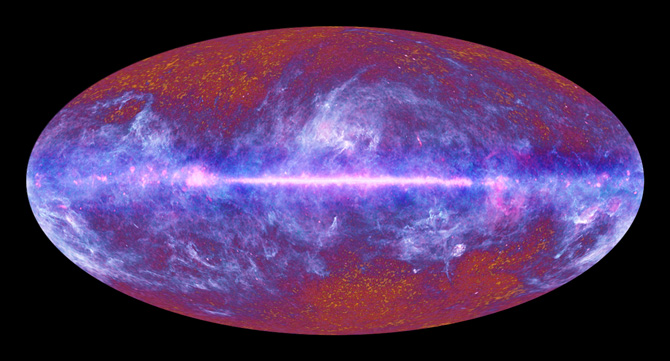
\includegraphics[scale=0.3]{figures/voids/planck_fullsky}
		\caption{A full sky map of the Cosmic Microwave Background as seen by the \textit{Planck} satellite [2010]}
		\label{fig:planck_fullsky}
\end{center}
\end{figure}

\section{LTB Model}

\section{Hierarchical Structure Formulation}

Structure formation is a highly non-linear process. It cannot be understand by the simple linear theory of wavelengths entering the horizon at different redshifts. However, numerical simulations are not the viable only line of attack. There exists an analytical framework centered around Smulochowski's work on fluctuations. The essential idea is that when we look at the ``entire universe", the matter density distribution shows no fluctuations. However, as we look at smaller and smaller scales, the fluctuations in the matter density $ \frac{\delta \rho }{\rho} $ increase and become more random. This variation of the density with scale can be viewed as a brownian walk - and this is where Smoluchowski's work comes into play.

%Now the critical density of a distribution of matter above which gravitational collapse overwhelms the background cosmological expansion varies with scale (... exactly why ?). 

The fluctuation spectrum is embedded in the initial conditions - at recombination - and depends on the inflationary model used. But essentially it can be fixed by hand, not worrying about what form of inflation created it. This initial condition then determines the future evolution of the matter density and halo formation. Even though the resulting evolution is statistical, it is not indeterminate. The distribution of halos at different redshifts depends on the fluctuation spectrum specified as part of the initial conditions.

The insights from the work on halo formation, from Press-Scheter to Sheth and Moreno, can be summarized as follows:

1. The halo size distribution as a function of redshift is a member of a statistical ensemble that is characterized by the initial conditions.

%2. Halo formation and growth is a highly non-linear process, which can be modeled accurately using Smulochowski's work on fluctuation theory.

3. Given a halo of a certain size at a certain redshift, one can trace its history backwards in time. As we decrease z, the halo shrinks, eventually reaching a point where its size is smaller than the critical density at that red-shift, and it then splits (most commonly into two pieces). Each branch can then be recursively processed to yield a fractal model of halo formation.

4. Halo formation exhibits scaling relations and universality. We can consider halos of mass m and m' and evaluate the corresponding critical densities of formation as a function of redshift. With an appropriate scaling we find that the two curves coincide.

Halo formation is a non-linear process, exhibiting self-similarity and universality!

The net effect of these considerations can be best summarized by Fig. \ref{fig:MilleniumSimulation} taken from \cite{Springel2006The-large-scale,Springel2005Simulating}.

\begin{figure}[hbtp]
	\centering
	\subfigure{
	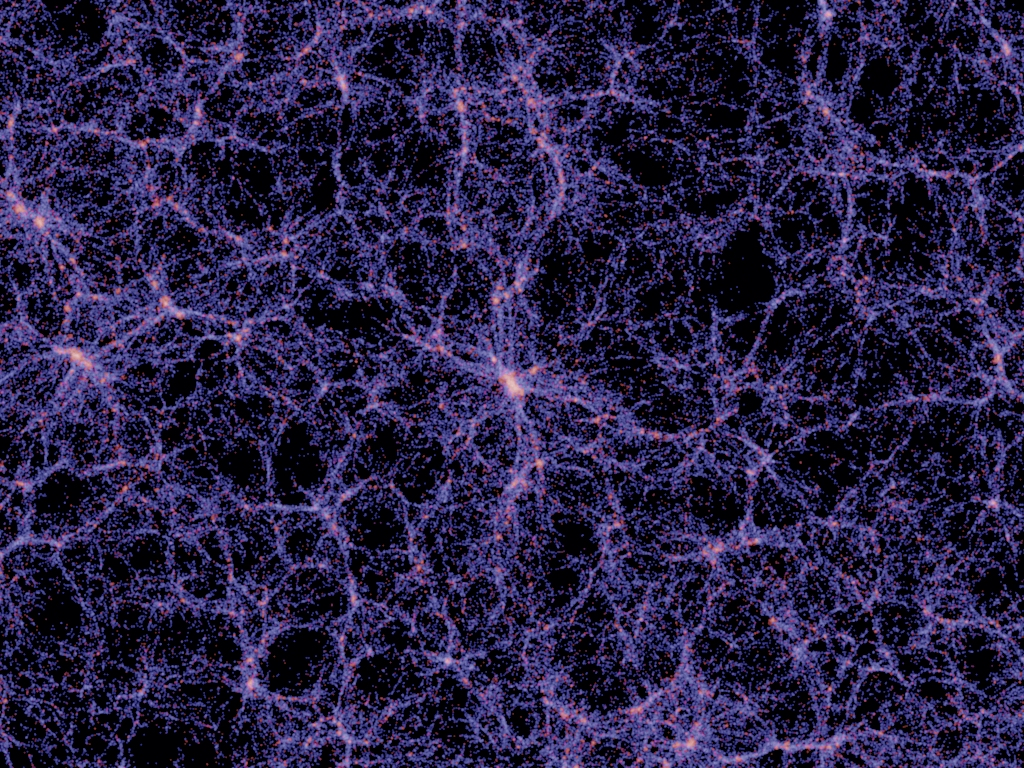
\includegraphics[scale=0.15]{figures/voids/galseq_D_063}
%	\label{fig:GalDistSim}
}
	\subfigure{
	\includegraphics[scale=0.15]{figures/voids/seqD_063a_half}
%	\label{fig:DarkMatterDistSim}
}
	\caption{The large scale distribution of visible matter (left) and dark matter (right) in the present epoch as modelled by the Millenium Simulation}
	\label{fig:MilleniumSimulation}
\end{figure}

\section{Cosmological Averaging}

Summarize Buchert and Wiltshire's work.

\section{Discussion}

There has been no lack of criticism of this model of apparent cosmic acceleration, much of which centers around the notion that our location near the center of a large void is in conflict with the cosmological principle and with precision cosmological measurements. For instance the abstract of one such rebuttal \cite{Moss2010Precision} begins with the statement that

"The suggestion that we occupy a privileged position near the centre of a large, nonlinear, and nearly spherical void has recently attracted much attention as an alternative to dark energy. ...."

In this and similar rebuttals the issue of our ``privileged position" near the center of a void is often raised as a philosophical objection to the model. However, contrary to common opinion, our location in the interior region of a void is not only likely but also necessary from an anthropic point of view. In fact, one can go on to argue that life-bearing systems are far more likely to occur in the relatively quiet interiors of voids rather than in the filaments or nodes of the cosmic web which are regions of star formation and hence full of highly energetic debris which would make the uninterrupted evolution of life on a planet over many eons unlikely.

Such an argument is amenable to experimental confirmation or rejection by looking at the results of the various exoplanetary searches in progress. In addition the results of void-finder models \cite{Colberg2008The-Aspen-Amsterdam} consistently show that \emph{the basic results of the various methods agree very well with each other in that they all locate a major void near the centre of our volume}.

Ultimately whether or not the void model rules out the existence of dark energy is not by itself the major issue at stake here. It is irrefutable that the inhomogeneous large-scale structure of the galactic web must figure into any complete analysis of CMB or other cosmological data.

%\end{doublespace}